\documentclass{anstrans}
%%%%%%%%%%%%%%%%%%%%%%%%%%%%%%%%%%%
\title{Coupled Neutronics and Microstructure Calculations to Model Radiation Damage in TREAT Fuel}
\author{Pedram Ghassemi, Sebastian Schunert, Daniel Schwen}
\institute{Idaho National Laboratory, Idaho Falls, ID}

\email{pghasse@ncsu.edu, sebastian.schunert@inl.gov, daniel.schwen@inl.gov}

%%%% packages and definitions (optional)
\usepackage{graphicx} % allows inclusion of graphics
\usepackage{booktabs} % nice rules (thick lines) for tables
\usepackage{microtype} % improves typography for PDF
\usepackage{algorithm}
\usepackage{algorithmic}
\usepackage{mathtools}
\usepackage{amsmath}

\input{./common/packages.tex}
\input{./common/def.tex}


\begin{document}
%%%%%%%%%%%%%%%%%%%%%%%%%%%%%%%%%%%%%%%%%%%%%%%%%%%%%%%%%%%%%%%%%%%%%%%%%%%%%%%%
\section{Introduction}
Radiation damage to structural materials and nuclear fuel is studied in a wide
range of scientific areas such as
nuclear power and semiconductor design \cite{basics}. Radiation damage
starts with the generation of a PKA (primary knock-on atom). This can occur due
to a nuclear reaction, radioactive decay, scattering,
etc. The method introduced focuses on radiation damage due to fission events.
There are several theoretical methods used to study radiation damage caused by
the ensuing cascade of secondary knock-on atoms.
Radiation transport theory can be used to assess displacement damage by describing
atomic motion in solids, but the governing equation for charged particles is difficult to solve.
Alternative methods include atomistic numerical models such as molecular dynamics
(MD) featuring the advantage that is it realistically treats the motion of atoms in a solid;
the downside is that it is computationally expensive. The binary collision approximation (BCA),
which assumes that the ion travels through a material by experiencing a series of
independent binary collisions, is commonly used to allow for efficient simulations.
A collision is treated by solving the classical scattering integral between two
colliding particles for the impact parameter of the incoming ion \cite{BCA}. It also
assumes that particles move in a straight path between collisions. Binary collision
Monte Carlo is used to simulate the avalanches caused by the PKAs due to fission.

Large scale effects of radiation on solids were observed in nuclear
fission reactors. There were noticeable structural and effects and it became
necessary to further investigate this physical occurrence.
Radiation damage can alter the physical and thermal
properties of solids and it is important to accurately model these effects to
satisfy safety limits.
Neutronics calculations will be fully coupled to the lower
length scale calculations to more accurately model this multi-physics phenomenon.

The goal of this work is enhancing the fidelity of radiation damage calculations
by using macroscopic high-fidelity neutronics calculations for computing the PKA
distribution. A coupled microscopic BCMC calculation uses these distributions obtained
at a number of sample points within the domain to sample the initial states of the PKAs.
The modeling will be done using applications from the MOOSE framework which was
developed at Idaho National Laboratory (INL). MAMMOTH, the reactor physics
application, performs the neutronics calculations and MARMOT, the microstructure
application, does the radiation damage calculations. Magpie is the glue application
that will allow MOOSE applications to link to and utilize various atomistic codes.

As an example, the effects of radiation damage on the TREAT fuel are analyzed. It is expected
that the damage will change thermal properties of the fuel such as the thermal
conductivity, heat capacity, and the density. Other results of interest are the
energy deposition distribution of fission fragments in the fuel and surrounding graphite.
Since the microstructure evolution will be coupled with neutronics calculations, it is
expected that the results will be more accurate than previous models.

%%%%%%%%%%%%%%%%%%%%%%%%%%%%%%%%%%%%%%%%%%%%%%%%%%%%%%%%%%%%%%%%%%%%%%%%%%%%%%%%
\section{Method}

The distribution of PKAs due to fission is calculated using the solution
from neutronics calculations.
Using the fission rates, $F$, from the transport calculations, the marginal
distribution with respect to the incident neutron energy can be computed. The fission
rate is defined as:
\begin{equation}
  F(\vr,E) = \Sigma_{f}(\vr,E) \phi(\vr,E) \Rightarrow F_{gi} = \Sigma_{f,gi} \phi_{g}
\end{equation}
where g is the energy group, and i is the target isotope.\\
The normalized marginal distribution is obtained by summing over all groups:
\begin{equation}
  F_i = \frac{\sum_{g=1}^G F_{gi} }{\sum_{g=1}^G \sum_{i=1}^I F_{gi}}
\end{equation}

A CDF can be computed from this marginal distribution and is sampled to
determine the target isotope.\\

Given a sampled target isotope, $i = i^*$, a conditional distribution, $F_g^c$, can be computed:
\begin{equation}
  F_g^c = \frac{F_{gi^*}}{\sum_{g=1}^G F_{gi^*} }
\end{equation}
A CDF is computed from this conditional distribution and is sampled
to determine the incident neutron energy.
The assumptions made for this method include:
\begin{itemize}
  \item Only be two fission products per fission
  \item The fission process is isotropic in the lab frame
  \item Momentum of the fission inducing neutron is neglected
  \item Momentum of the fission product
  neutrons is neglected
\end{itemize}

In order to tally the PKA distribution from fission, the fission yields
will be sampled with respect to the incident neutron energy
and the target. Since only the energy group, g, is known within a multigroup setting,
the incident neutron energy is obtained by sampling uniformly between $E_{g^*+1}$ and $E_{g^*}$.
Fission yield data is given for general energy ranges:\\

\begin{tabular}{  l  r }
  Thermal:    & $\le$ 0.5 eV \\
  Epithermal: & 0.5 eV $<$ E $\le$ 0.75 MeV \\
  Fast:       & 0.75 MeV $<$ E $\le$ 7 MeV \\
  High:       & $>$ 7 MeV \\
\end{tabular}

\vspace{0.5cm}
\noindent This data will be taken from ENDF libraries. \\

Given the target isotope and its energy range, the fission products (or PKAs)
can be determined by sampling a CDF that will be built from the fission yield data.
Each PKA can be defined by its atomic number (Z), mass number (A), energy (E),
and direction of motion ($\Omega$).\\
The PDF is defined as:
\begin{equation}
  P_{gi}(Z,A) = \frac{Y_{gi}(Z,A)}{\sum_{Z,A} Y_{gi}(Z,A)}
\end{equation}
where, $Y_{gi}(Z,A)$, is the yield of fission product isotope (Z,A) given energy range, g, and target isotope, i.

\begin{figure}[ht] % replace 't' with 'b' to force it to be on the bottom
  \centering
  \includegraphics[scale=0.4]{./figures/fission_product_yields.pdf}
  \caption{Fission sum yield distribution from ENDF}
\end{figure}

A CDF is computed and is sampled to determine the fission product isotope (Z,A).

The average kinetic energy of the fission products can be calculated using an empirical relationship
on both Z and A of the target isotope \cite{geant}:
\begin{equation}
  <T_{kin}> = 0.1178 \frac{Z_{target}^2}{A_{target}^{1/3}} + 5.8
\end{equation}

Once a single fission product is known, the other's mass number can be determined by invoking conservation of mass:
\begin{equation}
  A_{2} = A_{target} - A_{1} - \bar \nu
\end{equation}
where $A_{2}$ is the mass number of the second fission product, $A_{target}$ is the mass number of the target nucleus, $A_{1}$ is the mass of the first fission product, and
$\bar \nu$ is the (integer) number of neutrons released during fission. $\bar \nu$ is sampled on the interval of the nearest integers less than and greater than $\nu$ and is weighted based on the true value of $\nu$.

Similarly, Z can be obtained by invoking conservation of charge:
\begin{equation}
  Z_{2} = Z_{target} - Z_{1}
\end{equation}
where $Z_{2}$ is the atomic number of the second fission product, $Z_{target}$ is the atomic number of the target, and $Z_{1}$ is the atomic number of the first fission product.

The energy of each fission product can be calculated using an energy and momentum balance.
\begin{eqnarray}
  <T_{kin}> &=& E_{1} + E_{2} \\
  \vec p_{1} &=& \vec p_{2}
\end{eqnarray}

Solving for the energy of each fission product,
\begin{eqnarray}
  E_{1} &=& <T_{kin}>\left(1 +  \frac{A_{1}}{A_{2}}\right)^{-1}\\
  E_{2} &=& \frac{A_{1}}{A_{2}}E_{1}
\end{eqnarray}

The direction of one fission product will be sampled uniformly and the second
fission product will travel in the opposite direction.

%%%%%%%%%%%%%%%%%%%%%%%%%%%%%%%%%%%%%%%%%%%%%%%%%%%%%%%%%%%%%%%%%%%%%%%%%%%%%%%%
\section{Results and Analysis}


%%%%%%%%%%%%%%%%%%%%%%%%%%%%%%%%%%%%%%%%%%%%%%%%%%%%%%%%%%%%%%%%%%%%%%%%%%%%%%%%
\subsection{(a) UO2 pellet - Graphite model}

%Below is a representation of the $UO_2$ pellet in the graphite.

%\begin{figure}[ht] % replace 't' with 'b' to force it to be on the bottom
%  \centering
%  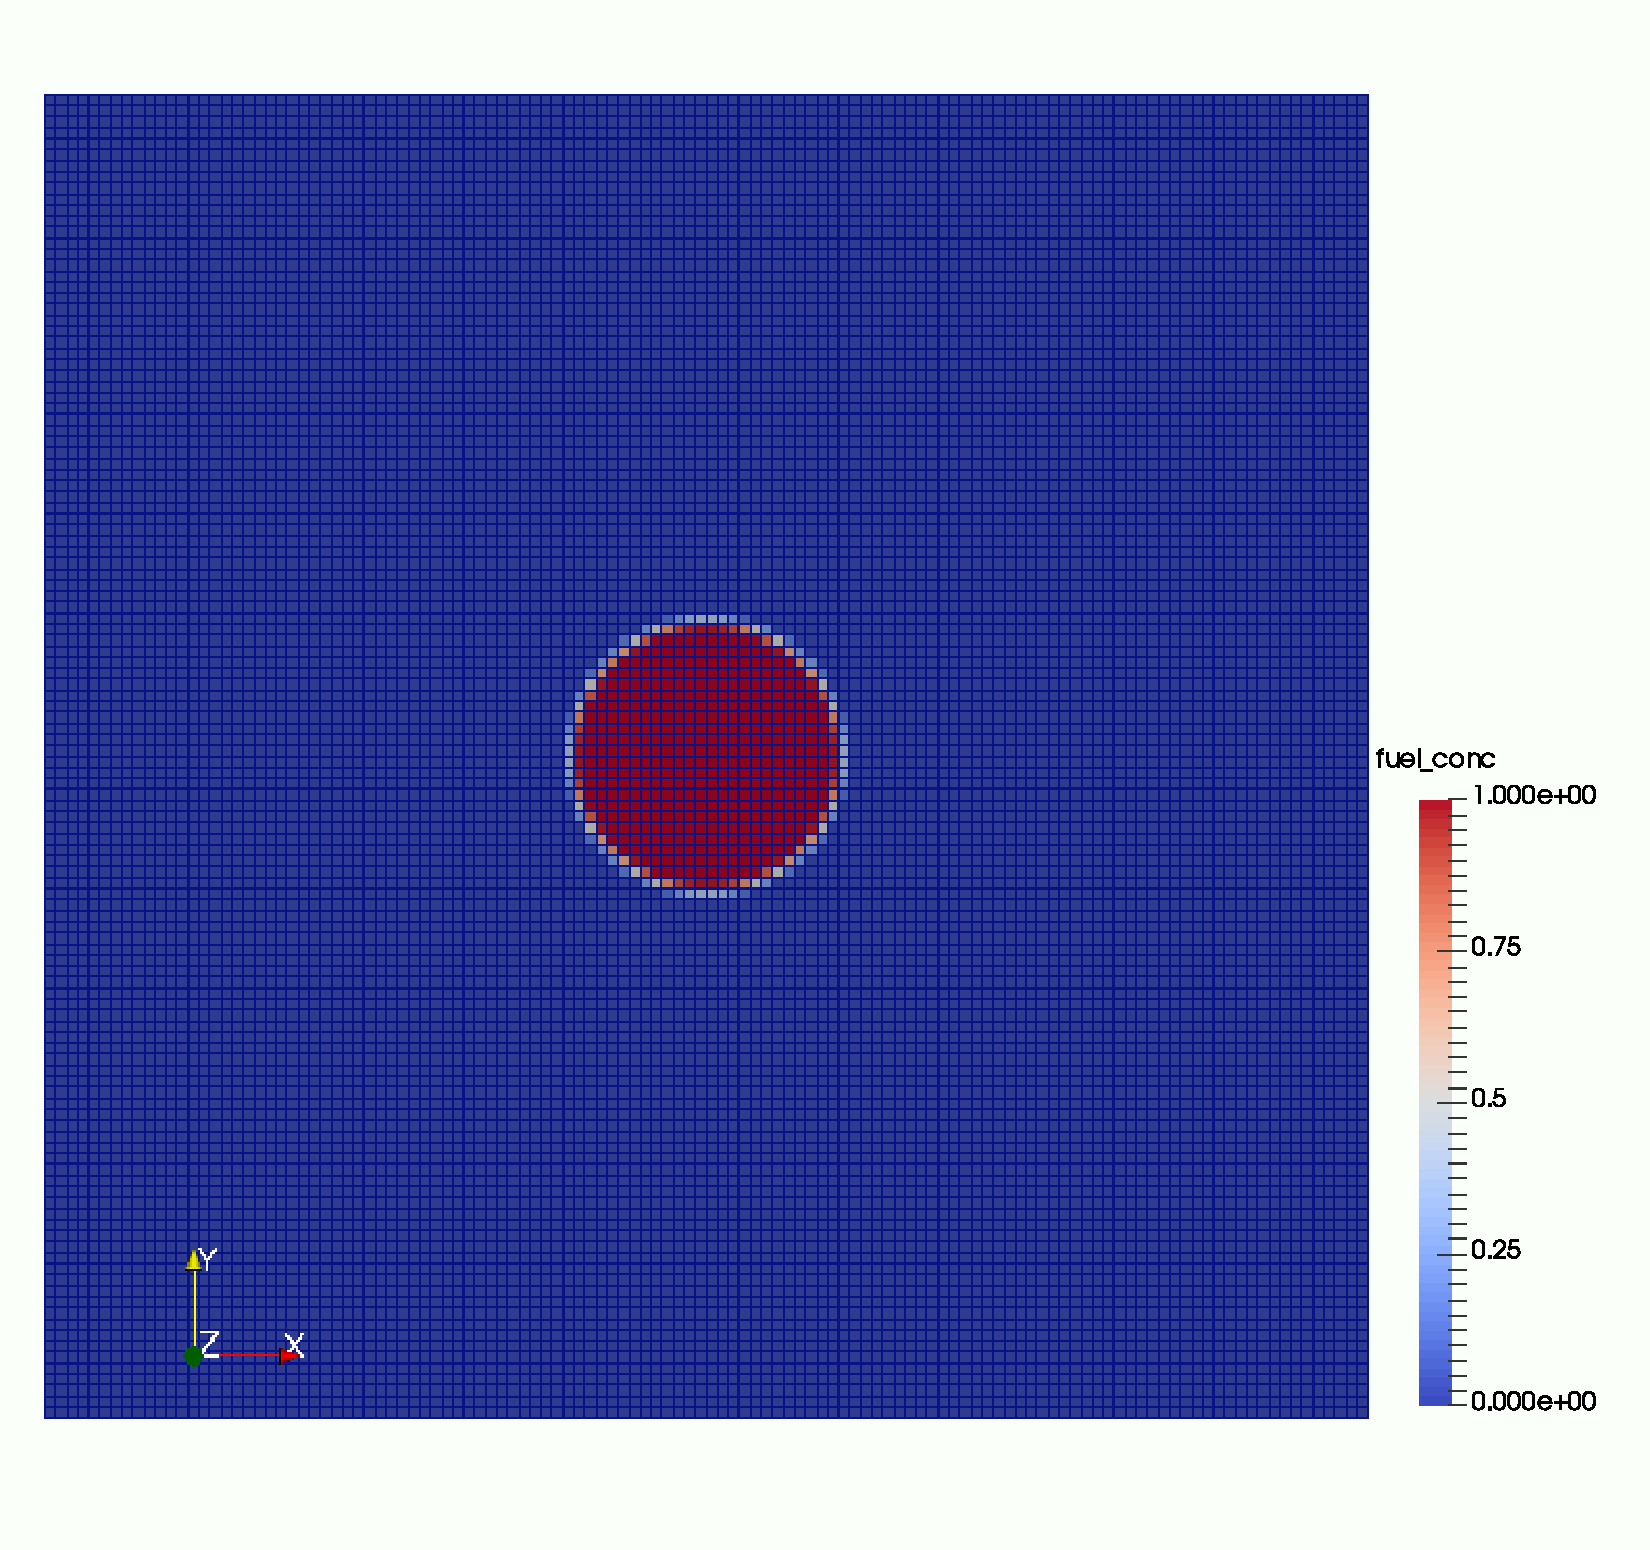
\includegraphics[scale=0.3]{./figures/fuel_conc2.pdf}
%  \caption{Initial condition of $UO_2$ pellet in graphite}
%\end{figure}


%%%%%%%%%%%%%%%%%%%%%%%%%%%%%%%%%%%%%%%%%%%%%%%%%%%%%%%%%%%%%%%%%%%%%%%%%%%%%%%%
\section{Conclusions}



%%%%%%%%%%%%%%%%%%%%%%%%%%%%%%%%%%%%%%%%%%%%%%%%%%%%%%%%%%%%%%%%%%%%%%%%%%%%%%%%
\appendix
\section{Appendix}

%Numbering in the appendix is different:
%\begin{equation} \label{eq:appendix}
%  2 + 2 = 5\,.
%\end{equation}
%and another equation:
%\begin{equation} \label{eq:appendix2}
%  a + b = c\,.
%\end{equation}

%%%%%%%%%%%%%%%%%%%%%%%%%%%%%%%%%%%%%%%%%%%%%%%%%%%%%%%%%%%%%%%%%%%%%%%%%%%%%%%%
\section{Acknowledgments}


%%%%%%%%%%%%%%%%%%%%%%%%%%%%%%%%%%%%%%%%%%%%%%%%%%%%%%%%%%%%%%%%%%%%%%%%%%%%%%%%
\bibliographystyle{ans}
\bibliography{bibliography}

\begin{thebibliography}{1}

\bibitem{basics} Mark T. Robinson {\em Basic physics of radiation damage production}
Journal of Nuclear Materials 216 (1994) 1-28 \\

\bibitem{BCA} R. Smith (ed.) {\em Atomic and ion collisions in solids and at surfaces:
 theory, simulation and applications}, Cambridge University Press, Cambridge, UK,
  1997 \\

\bibitem{geant} GEANT4 Physics Manual Version: 10.2 (4 December 2015)

\end{thebibliography}



\end{document}
